\documentclass{article}

\usepackage{framed}
\usepackage[margin=2.2cm]{geometry}
\usepackage{graphicx}
\usepackage{hyperref}
\usepackage{lscape}
\usepackage{listings}
\usepackage{tikz}
\usetikzlibrary{fit}
\usepackage{verbatim}


\renewcommand{\familydefault}{\sfdefault}

\setlength{\tabcolsep}{20pt}
\renewcommand{\arraystretch}{2}

\newcommand{\fignote}[1]{{\small{#1}}}

\title{A gentle introduction to data visualization in R for TAP Striking
  Statistics}
\date{March 2020}

\begin{document}
\maketitle

\section{Goals of this tutorial}

It is often easier and quicker to communicate coding concepts
    in an interactive in-person workshop. We are unlikely to have that
    opportunity soon. The idea of this tutorial is to share a full
    R worlflow of a striking stat we have already started discussing in
    Teams. I have also shared online guides that I believe give a good
    introduction to key topics. Hopefully, you would be able to go
    back and forth between the guides, which give a conceptual overview
    of R, and the example code of our own striking stat, which
    provides an opportunity to directly apply the new concepts. That
    self-guided process will be enhanced by a Webex Q\&A whenever convenient.

 Figure \ref{fig_stat} shows the current version of the striking stat
 (using Tanou's export data) and a possible publication-ready version.\\
 
I have selected resources and examples with two goals in mind:
\begin{enumerate}
\item You can explore examples with enough background information to
  get a fair feel for the possibilities and challenges of data
  visualization in R
  \item We have enough of a shared understanding to jointly edit the
    occasional visualation, even if we use mostly use different
    tools

    \begin{framed}
    For example, a few weeks ago we needed to change a couple
    of maps to represent Western Sahara. Alexis had the correct
    shapefiles; Hannah and I had two different maps produced with two
    different workflows. If we had been a bit more coordinated,
    changing the underlying maps would have involved one line of reproducible
    code. (See example \url{5_plot_wb_world_map.R}). As it was, Hannah and I painted
    over our existing maps in Microsoft Paint.
  \end{framed}
\end{enumerate}
    
  \textbf{This is not}
\begin{itemize}
\item  A comprehensive introduction to R, to
      data visualization or even to data visualization in R
\item (Yet {\tt:-)}) An evangelistic mission to convert everyone to R
  
\end{itemize}


\section{Why R for data visualization?}

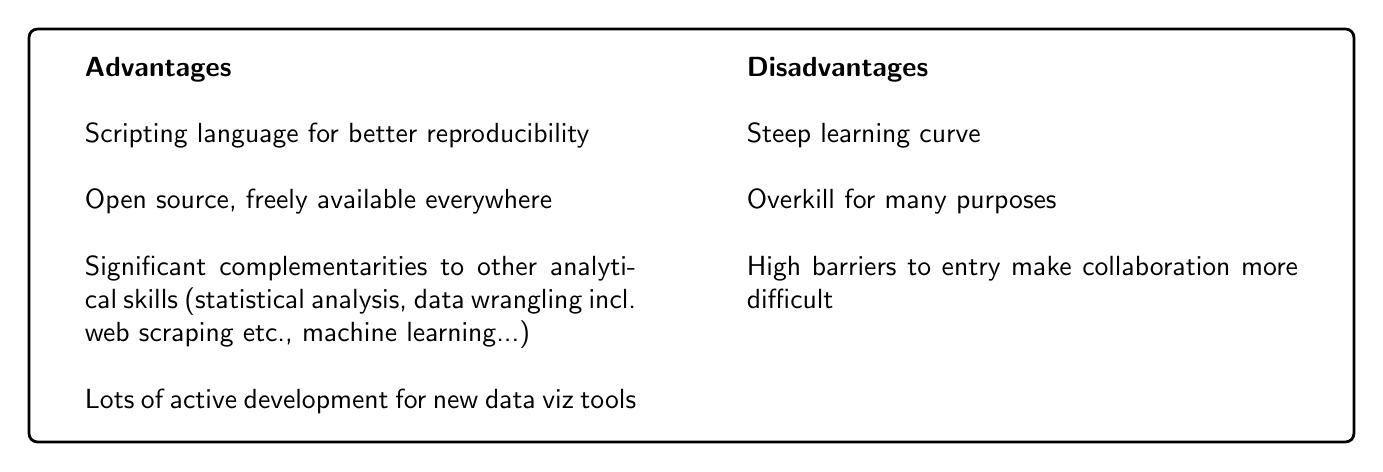
\begin{tikzpicture}
 \node[inner sep=0pt] (tab){%
\begin{tabular}[hbt]{p{7cm}p{7cm}}

  \textbf{Advantages} & \textbf{Disadvantages} \\
  Scripting language for better reproducibility & Steep
                                                               learning
                             curve\\
  Open source, freely available everywhere & Overkill for many
                                             purposes\\
  
  Significant complementarities to other analytical skills
  (statistical analysis, data wrangling incl. web scraping etc.,
  machine learning...)&High barriers to entry make collaboration more difficult\\
  Lots of active development for new data viz tools &\\

\end{tabular}
};
\node[draw=black, inner sep=0pt, rounded corners=3pt, line width=1pt,
fit=(tab.north west) (tab.north east) (tab.south east) (tab.south west)] {};
\end{tikzpicture}

%\vspace{2em}

% \textbf{Who else is using R?}
% \url{https://github.com/ThinkR-open/companies-using-r} and see Figure \ref{fig_useR}


% \begin{figure}
%   \caption{Jobs and scholarly articles using different programming
%     languages in 2018}
%   \label{fig_useR}
  
%   \includegraphics[width =  0.47\textwidth]{pictures/number_of_scholarly_articles}%
%   \includegraphics[width =
%   0.53\textwidth]{pictures/number_of_data_science_jobs}
%   \smallskip
%   \fignote{\emph{Source} \url{http://r4stats.com/articles/popularity/}}

% \end{figure}


\section{Basic setup}
\begin{itemize}
\item Download and install R from the R-project website
  \url{https://www.r-project.org/about.html}


  \item Download and install the free version of RStudio
    \url{https://rstudio.com/products/rstudio/download/}

  \item Once in R, install the tidyverse package

    \begin{lstlisting}
      install.packages(``tidyverse'')
  \end{lstlisting}
  
  Please follow the defaults unless you have a good reason not to.

  \item  All code and material for this tutorial can be downloaded here \url{https://github.com/ammapanin/striking-statistics-tap/tree/master/R-for-TAP}
\end{itemize}

\section{Outline of this tutorial}

\begin{enumerate}
\item Open \url{1_plot_simple_export_bars.R}
  Run the code and produce your first plot! Don't worry about
  understanding each command.

  \item Read through the tutorial on 'Data Types and Structures' at
    the following link
    \url{https://swcarpentry.github.io/r-novice-inflammation/13-supp-data-structures/index.html}

    \item Go back to  \url{1_plot_simple_export_bars.R}
  Try to understand the different data types that can already be found
  in the code. Get more familiar with the dataset and the plotting options.

 
  \item Read through this chapter introducing ggplot
    \url{https://r4ds.had.co.nz/data-visualisation.html}

      \item Read about dply rbasics
    \url{https://r4ds.had.co.nz/transform.html}

    
  \item Open \url{2_plot_intermediate_export_bars.R}

    Get familiar with some of the customizations that are offered in
    this script. Again, don't worry if some pieces of code don't make
    complete sense.
    
      \item Then read more about 'Understanding Factors'. Factors are a
    specific data type for storing categorical variables. You would
    eventually need to be comfortable with them as they are important
    for plotting (e.g. ordering country labels)
    
    \url{https://swcarpentry.github.io/r-novice-inflammation/12-supp-factors/index.html}
    
       \item Then attempt to create the final graphic with \url{3_plot_advanced_export_bars.R}
      Look for your output in the main project folder. It will be
      called something like \url{E4T_export_compliance.png}

      \item Go through \url{4_tidy_downloaded_data.R} to look under
        the hood at the data cleaning and transformation
        process to go from the World Bank download to the tidy dataset
        we used for analysis
\end{enumerate}

\newpage
\begin{landscape}
  \begin{figure}
    \caption{A striking stat to be customized in R}
    \label{fig_stat}
 \includegraphics[width =  0.5\linewidth]{pictures/time_to_export_v1}
   \includegraphics[width =
   0.5\linewidth]{pictures/E4T_export_compliance}
  \end{figure}

\end{landscape}

%\section{Additional resources}


\end{document}


%%% Local Variables:
%%% mode: latex
%%% TeX-master: t
%%% End:
